\documentclass[12pt]{article}
\usepackage[margin=2.5cm]{geometry}
\usepackage{enumerate}
\usepackage{amsfonts}
\usepackage{amsmath}
\usepackage{fancyhdr}
\usepackage{amsmath}
\usepackage{amssymb}
\usepackage{amsthm}
\usepackage{mdframed}
\usepackage{graphicx}
\usepackage{subcaption}
\usepackage{soul}

\begin{document}
\title{Worksheet 20 Solution}
\author{Hyungmo Gu}
\maketitle

\section*{Question 1}
\begin{enumerate}[a.]
    \item

    \bigskip

    \begin{proof}

    Let $V = \{1,2,3,4,5,6\}$, $E = \{(1,2),(1,6),(2,3),(3,4),(4,5),(5,6)\})$.

    \bigskip

    We need to prove the graph $G = (V,E)$ is bipartite by proving the following
    properties:

    \begin{enumerate}[1.]
        \item There exists subsets $V_1, V_2 \subset V$ such that
        $V_1 \neq \emptyset, V_2 \neq \emptyset$, and $V_1$ and $V_2$ form
        a partition of $V$.
        \item Every edge in $E$ has exactly one endpoint in $V_1$ and one in $V_2$.
    \end{enumerate}

    \bigskip

    We will prove the properties in parts.

    \bigskip

    \ul{\textbf{Part 1 (Proving $V_1 \neq \emptyset, V_2 \neq \emptyset$,
    and $V_1$ and $V_2$ form a partition of $V$):}}

    \bigskip

    Let $V_1 = \{1,3,5\}$ and $V_2 = \{2,4,6\}$.

    \bigskip

    We need to prove $V_1 \neq \emptyset, V_2 \neq \emptyset$, and
    $V_1$ and $V_2$ form a partition of $V$, i.e $V_1 \cup V_2 = V
    \land V_1 \cap V_2 = \emptyset$.

    \bigskip

    First, we need to show the subsets $V_1$ and $V_2$ are non-empty.

    \bigskip

    The header tells us both subsets $V_1$ and $V_2$ have more than
    1 elements.

    \bigskip

    Then, using these facts, we can conclude $V_1 \neq \emptyset$ and
    $V_2 \neq \emptyset$.

    \bigskip

    Finally, we need to show $V_1 \cup V_2 = V$ and $V_1 \cap V_2 = \emptyset$.

    \bigskip

    The header tells us $V_1 = \{1,3,5\}$ and $V_2 = \{2,4,6\}$.

    \bigskip

    Then, we can calculate

    \begin{align}
        V_1 \cup V_2 &= \{1,2,3,4,5,6\} = V\\
        V_1 \cap V_2 &= \emptyset
    \end{align}

    \bigskip

    \ul{\textbf{Part 2 (Proving every edge in $E$ has exactly one endpoint
    in $V_1$ and\\ one in $V_2$):}}

    \bigskip

    Let $V_1 = \{1,3,5\}$ and $V_2 = \{2,4,6\}$.

    \bigskip

    We need to show every edge in $E$ has exactly one endpoint in $V_1$ and
    one in $V_2$.

    \bigskip

    The header tells us $V_1 = \{1,3,5\}$, $V_2 = \{2,4,6\}$,
    and $E = \{(1,2),(1,6),(2,3),\\(3,4),(4,5),(5,6)\})$.

    \bigskip

    Using these facts, we can generate the following table.

    \bigskip

    \begin{tabular}{|c|p{3cm}|c|p{3cm}|}
        \hline
        Edge (1,2) & - 1 is in $V_1$ \newline - 2 is in $V_2$ & Edge (3,4) & - 3 is in $V_1$ \newline - 4 is in $V_2$\\
        \hline
        Edge (1,6) & - 1 is in $V_1$ \newline - 6 is in $V_2$ & Edge (4,5) & - 4 is in $V_2$ \newline - 6 is in $V_1$\\
        \hline
        Edge (2,3) & - 2 is in $V_2$ \newline - 3 is in $V_1$ & Edge (5,6) & - 5 is in $V_1$ \newline - 6 is in $V_2$\\
        \hline
    \end{tabular}

    \bigskip

    Then, it follows from observation that every edge in $E$ has
    one endpoint in $V_1$ and one in $V_2$.

    \end{proof}

    \bigskip

    \begin{mdframed}
        \underline{\textbf{Pseudoproof:}}

        \bigskip

        Let $V = \{1,2,3,4,5,6\}$, $E = \{(1,2),(1,6),(2,3),(3,4),(4,5),(5,6)\})$.

        \bigskip

        We need to prove the graph $G = (V,E)$ is bipartite by proving the following
        properties:

        \begin{enumerate}[1.]
            \item There exists subsets $V_1, V_2 \subset V$ such that
            $V_1 \neq \emptyset, V_2 \neq \emptyset$, and $V_1$ and $V_2$ form
            a partition of $V$.
            \item Every edge in $E$ has exactly one endpoint in $V_1$ and one in $V_2$.
        \end{enumerate}

        \bigskip

        We will prove the properties in parts.

        \bigskip

        \begin{enumerate}[1.]
            \item Show there exists subsets $V_1, V_2 \subset V$ such that
            $V_1 \neq \emptyset, V_2 \neq \emptyset$, and $V_1$ and $V_2$ form
            a partition of $V$

            \bigskip

            Let $V_1 = \{1,3,5\}$ and $V_2 = \{2,4,6\}$.

            \bigskip

            We need to prove $V_1 \neq \emptyset, V_2 \neq \emptyset$, and
            $V_1$ and $V_2$ form a partition of $V$, i.e $V_1 \cup V_2 = V
            \land V_1 \cap V_2 = \emptyset$.

            \bigskip

            \begin{enumerate}[1.]
                \item Show $V_1 \neq \emptyset, V_2 \neq \emptyset$

                First, we need to show the subsets $V_1$ and $V_2$ are non-empty.

                \begin{mdframed}
                The header tells us both subsets $V_1$ and $V_2$ have more than
                1 elements.

                \bigskip

                Then, using these facts, we can conclude $V_1 \neq \emptyset$ and
                $V_2 \neq \emptyset$.

                \end{mdframed}

                \item Show $V_1 \cup V_2 = V \land V_1 \cap V_2 = \emptyset$

                \bigskip

                Second, we need to show $V_1 \cup V_2 = V$ and $V_1 \cap V_2 = \emptyset$.

                \bigskip

                \begin{mdframed}
                The header tells us $V_1 = \{1,3,5\}$ and $V_2 = \{2,4,6\}$.

                \bigskip

                Then, we can calculate

                \begin{align}
                    V_1 \cup V_2 &= \{1,2,3,4,5,6\} = V\\
                    V_1 \cap V_2 &= \emptyset
                \end{align}

                \end{mdframed}

            \end{enumerate}

            \bigskip

            \begin{mdframed}
            \underline{\textbf{Part 1:}}

            \bigskip

            Let $V_1 = \{1,3,5\}$ and $V_2 = \{2,4,6\}$.

            \bigskip

            We need to prove $V_1 \neq \emptyset, V_2 \neq \emptyset$, and
            $V_1$ and $V_2$ form a partition of $V$, i.e $V_1 \cup V_2 = V
            \land V_1 \cap V_2 = \emptyset$.

            \bigskip

            First, we need to show the subsets $V_1$ and $V_2$ are non-empty.

            \bigskip

            The header tells us both subsets $V_1$ and $V_2$ have more than
            1 elements.

            \bigskip

            Then, using these facts, we can conclude $V_1 \neq \emptyset$ and
            $V_2 \neq \emptyset$.

            \bigskip

            Finally, we need to show $V_1 \cup V_2 = V$ and $V_1 \cap V_2 = \emptyset$.

            \bigskip

            The header tells us $V_1 = \{1,3,5\}$ and $V_2 = \{2,4,6\}$.

            \bigskip

            Then, we can calculate

            \begin{align}
                V_1 \cup V_2 &= \{1,2,3,4,5,6\} = V\\
                V_1 \cap V_2 &= \emptyset
            \end{align}
            \end{mdframed}

            \item Show every edge in $E$ has exactly one endpoint in $V_1$ and one in $V_2$.

            \bigskip

            Let $V_1 = \{1,3,5\}$ and $V_2 = \{2,4,6\}$.

            \bigskip

            We need to show every edge in $E$ has exactly one endpoint in $V_1$ and
            one in $V_2$.

            \bigskip

            \begin{mdframed}

            The header tells us $V_1 = \{1,3,5\}$, $V_2 = \{2,4,6\}$,
            and $E = \{(1,2),(1,6),(2,3),\\(3,4),(4,5),(5,6)\})$.

            \bigskip

            Using these facts, we can generate the following table.

            \bigskip

            \begin{tabular}{|c|p{3cm}|c|p{3cm}|}
                \hline
                Edge (1,2) & - 1 is in $V_1$ \newline - 2 is in $V_2$ & Edge (3,4) & - 3 is in $V_1$ \newline - 4 is in $V_2$\\
                \hline
                Edge (1,6) & - 1 is in $V_1$ \newline - 6 is in $V_2$ & Edge (4,5) & - 4 is in $V_2$ \newline - 6 is in $V_1$\\
                \hline
                Edge (2,3) & - 2 is in $V_2$ \newline - 3 is in $V_1$ & Edge (5,6) & - 5 is in $V_1$ \newline - 6 is in $V_2$\\
                \hline
            \end{tabular}

            \bigskip

            Then, it follows from observation that every edge in $E$ has
            one endpoint in $V_1$ and one in $V_2$.

            \end{mdframed}

            \bigskip

            \begin{mdframed}

            \underline{\textbf{Part 2:}}

            \bigskip

            Let $V_1 = \{1,3,5\}$ and $V_2 = \{2,4,6\}$.

            \bigskip

            We need to show every edge in $E$ has exactly one endpoint in $V_1$ and
            one in $V_2$.

            \bigskip

            The header tells us $V_1 = \{1,3,5\}$, $V_2 = \{2,4,6\}$,
            and $E = \{(1,2),(1,6),(2,3),\\(3,4),(4,5),(5,6)\})$.

            \bigskip

            Using these facts, we can generate the following table.

            \bigskip

            \begin{tabular}{|c|p{3cm}|c|p{3cm}|}
                \hline
                Edge (1,2) & - 1 is in $V_1$ \newline - 2 is in $V_2$ & Edge (3,4) & - 3 is in $V_1$ \newline - 4 is in $V_2$\\
                \hline
                Edge (1,6) & - 1 is in $V_1$ \newline - 6 is in $V_2$ & Edge (4,5) & - 4 is in $V_2$ \newline - 6 is in $V_1$\\
                \hline
                Edge (2,3) & - 2 is in $V_2$ \newline - 3 is in $V_1$ & Edge (5,6) & - 5 is in $V_1$ \newline - 6 is in $V_2$\\
                \hline
            \end{tabular}

            \bigskip

            Then, it follows from observation that every edge in $E$ has
            one endpoint in $V_1$ and one in $V_2$.

            \end{mdframed}

        \end{enumerate}

    \end{mdframed}

    \item

    Let $G = (V,E)$ be a complete bipartite graph.

    \bigskip

    Then, by property 3, we can conclude each vertex in $V_1$ is adjacent to all
    verticies in $V_2$.

    \bigskip

    Since there are $n$ many edges for each vertex in $V_1$, and since there are $m$
    many verticies in $V_1$, we can calculate that the vertices in $V_1$ has

    \setcounter{equation}{0}
    \begin{align}
        nm
    \end{align}

    edges.

    \bigskip

    Then, since there are no new edges for each vertex in $V_2$, we can conclude
    the graph has $nm$ edges.

    \item

    \textbf{Conjecture:} If a set of verticies forms a cycle in a graph G and G is bipartite, then
    the length of the set of verticies is even. (i.e. $\forall G = (C,E), Cycle(G) \land Bipartite(G) \Rightarrow \exists k \in \mathbb{Z}, \lvert C \rvert = 2k$)

    \bigskip

    \underline{\textbf{Pseudoproof:}}

    \bigskip

    Strategy: prove by contraposition.

    \bigskip

    Let $G$ be a graph with set of verticies $C$ and edges $E$. Assume the length
    of $C$ is odd.

    \bigskip

    We need to prove the graph is not bipartite.

    \bigskip

    \begin{enumerate}[1.]
        \item .
    \end{enumerate}

    \underline{\textbf{Notes:}}

    \begin{itemize}
        \item Cycle with odd number of verticies - Not bipartite

        % \begin{center}
        % 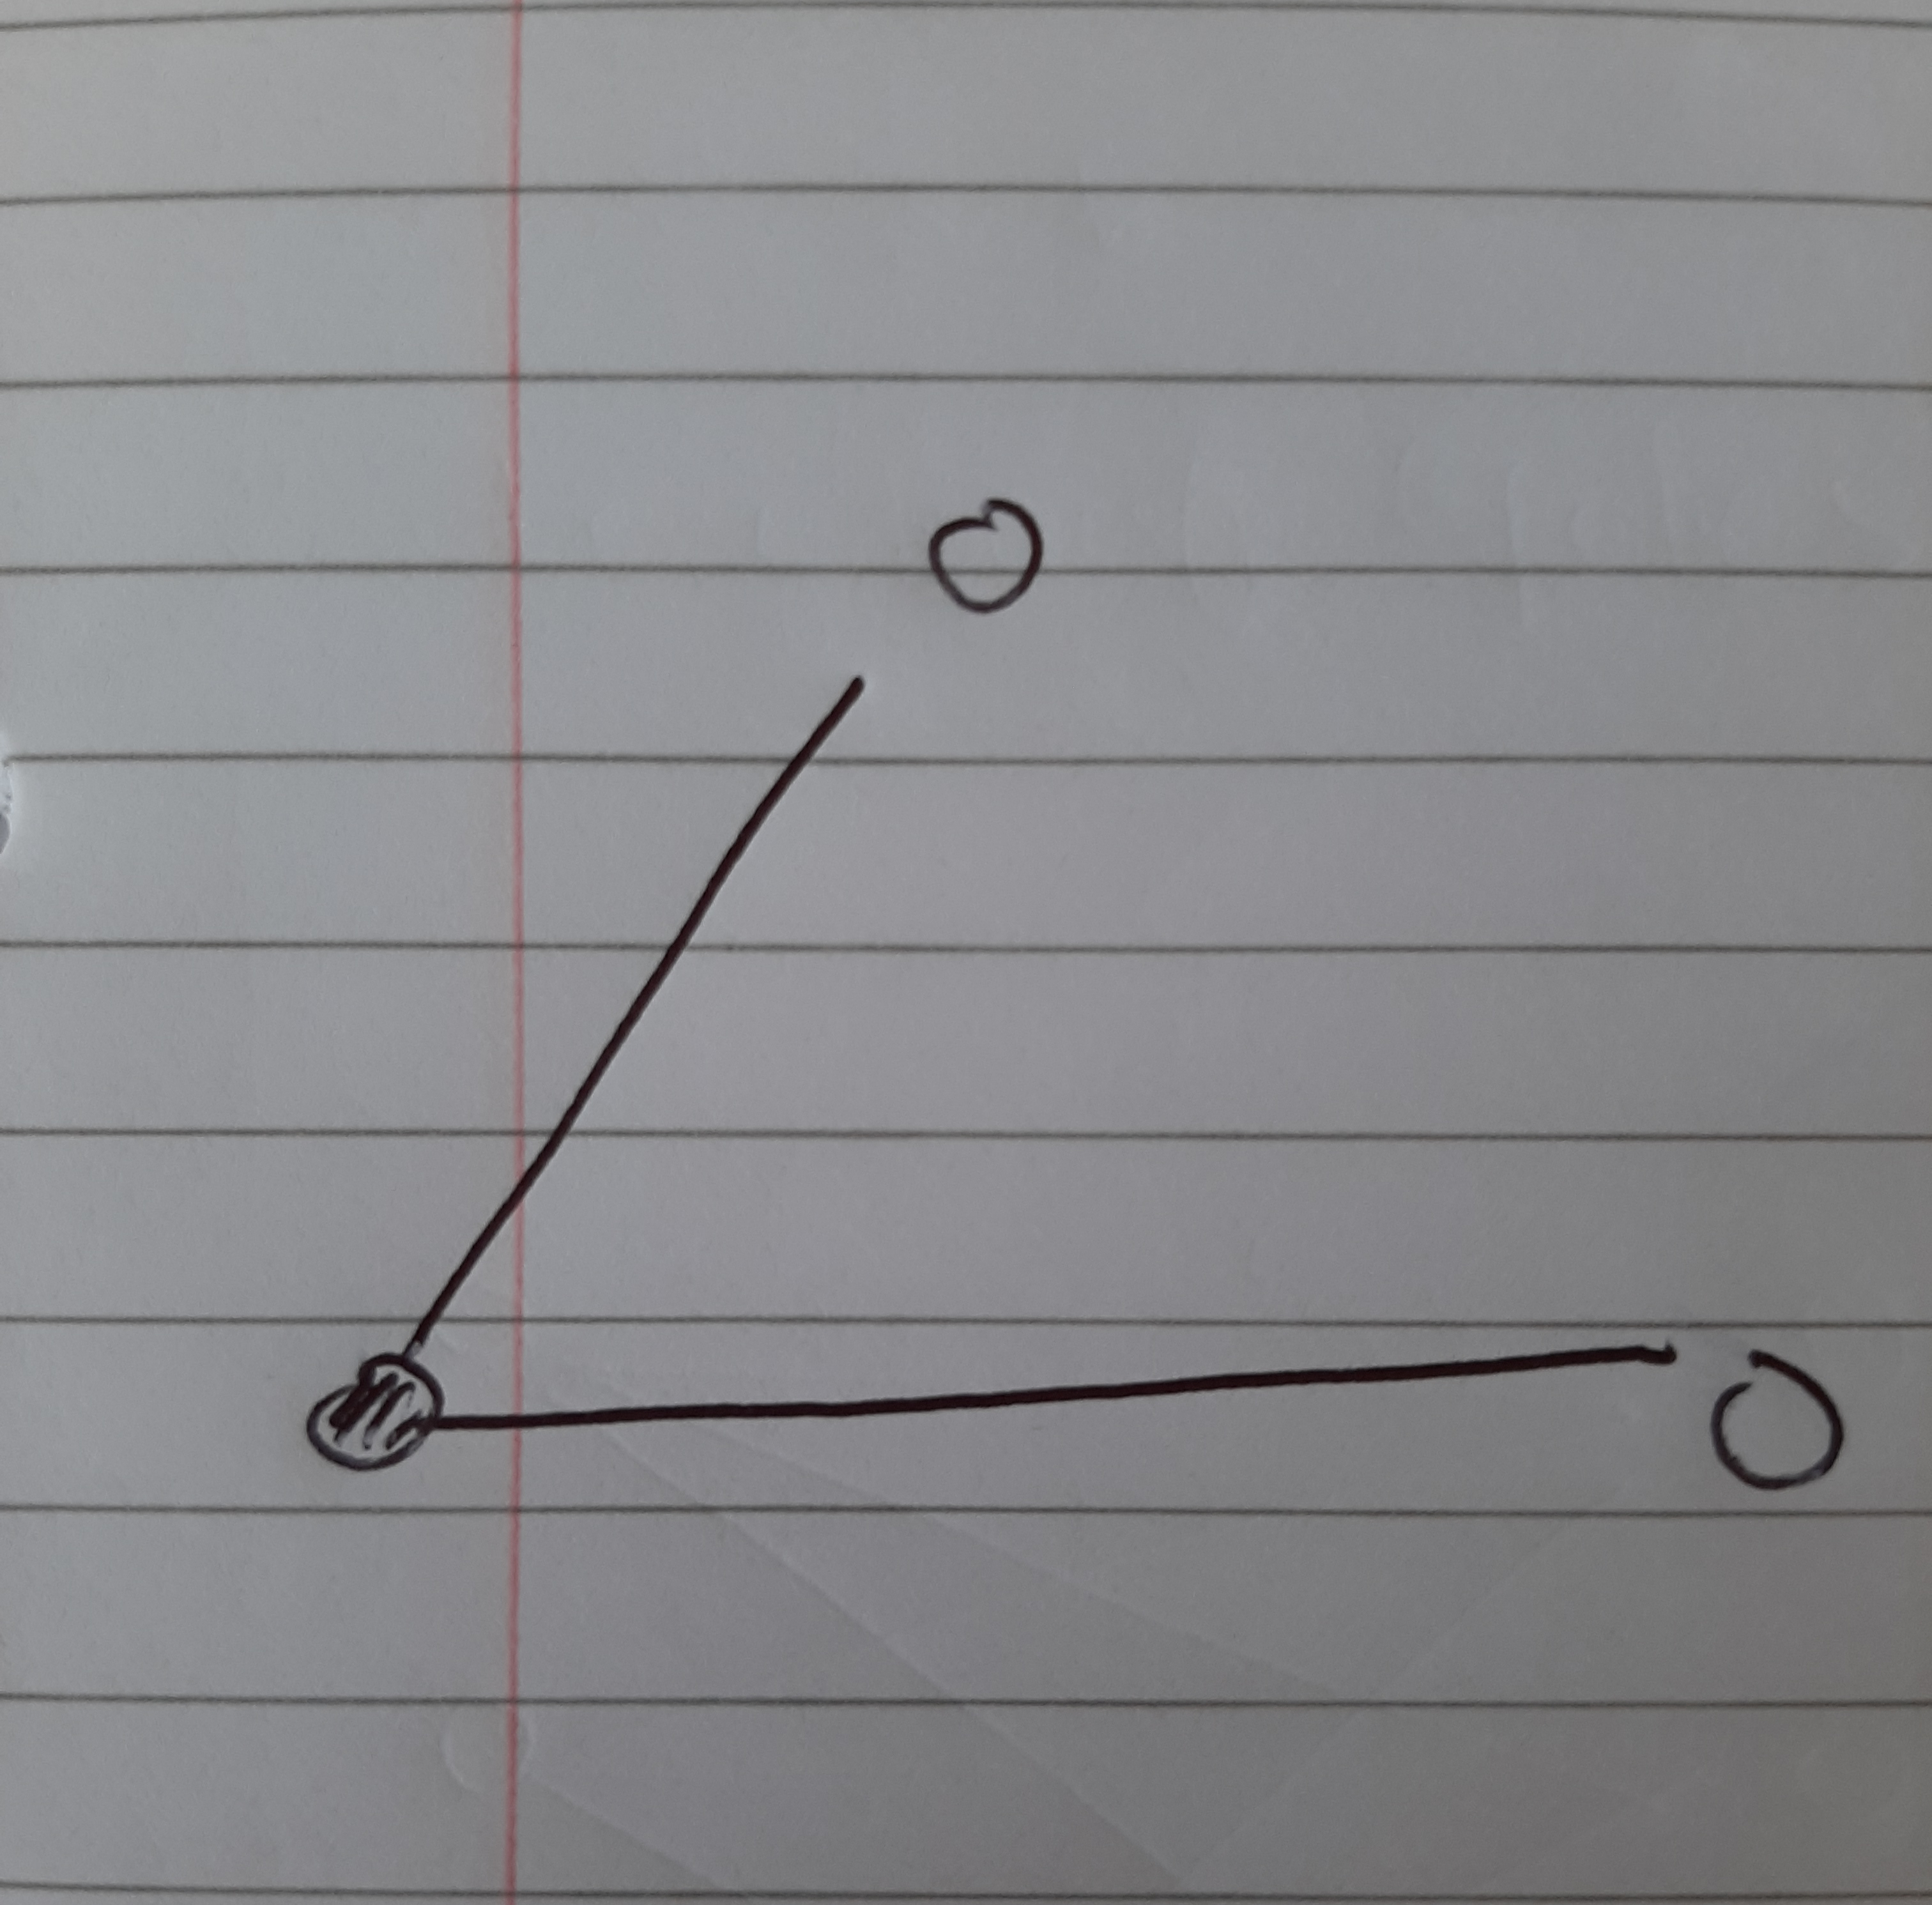
\includegraphics[width=0.4\linewidth]{images/worksheet_20_q1c_comments_1.jpg}
        % \end{center}

        \item Cycle with even number of verticies - Bipartite

        % \begin{center}
        % 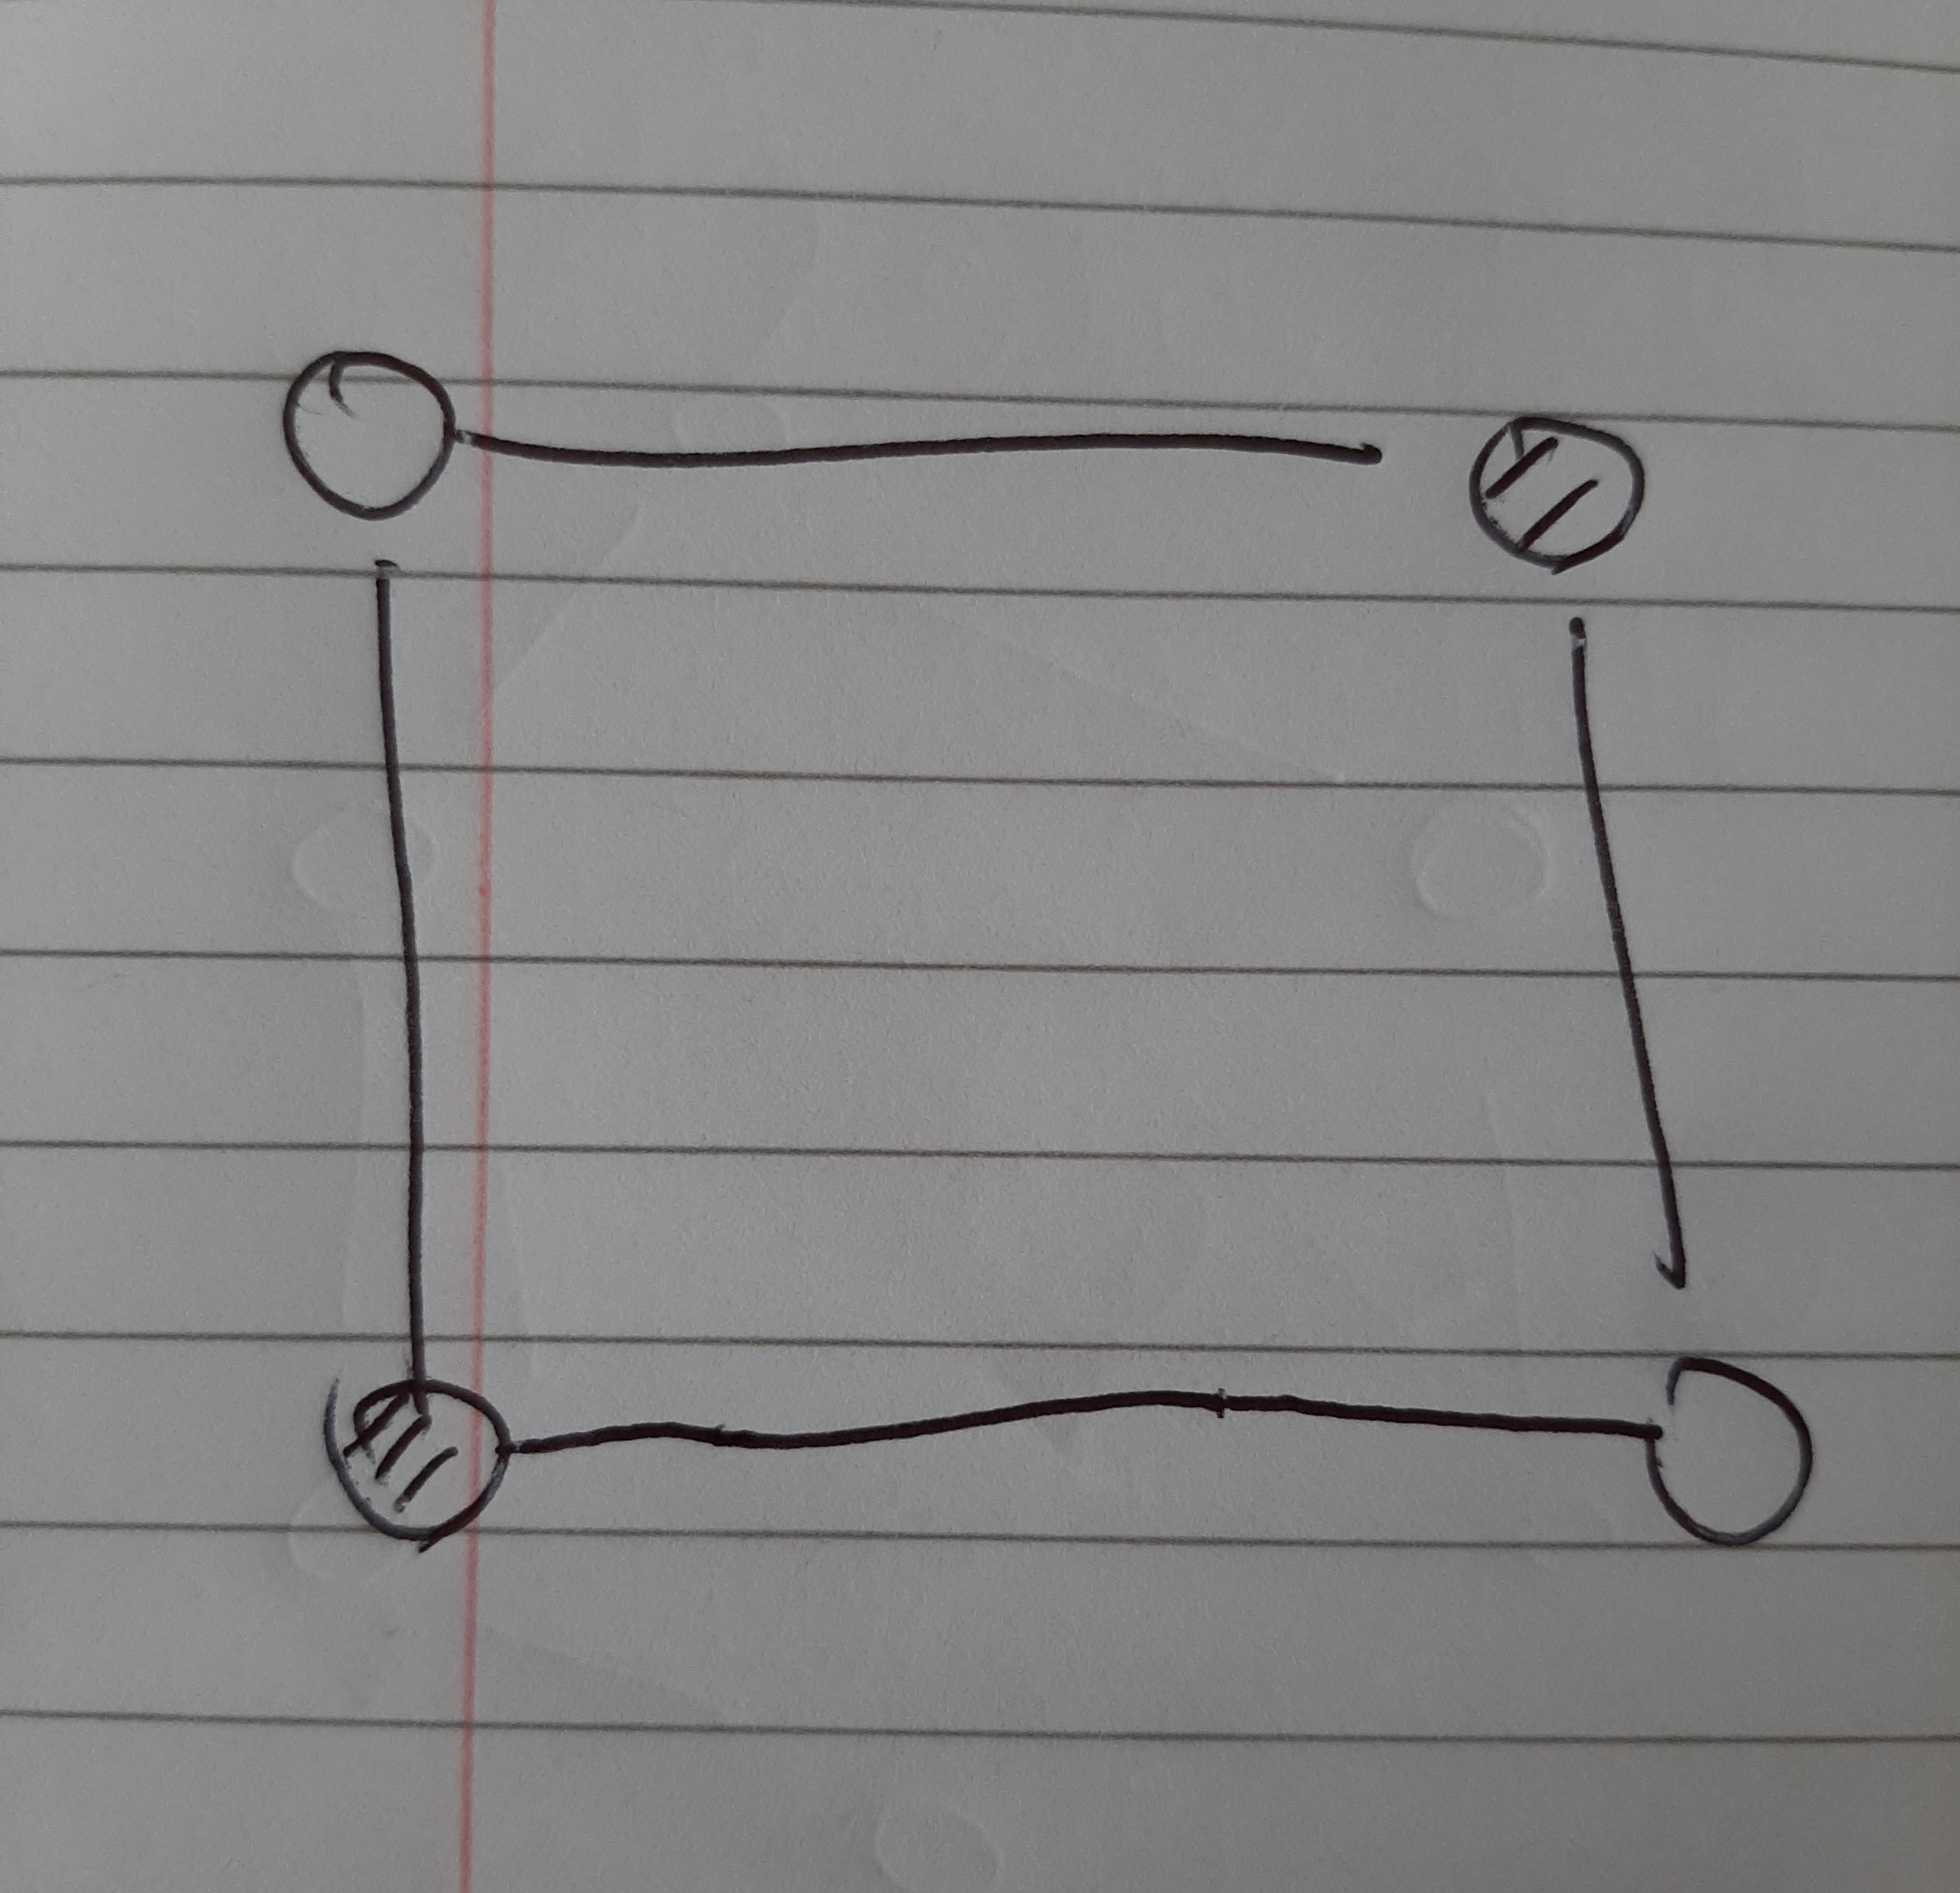
\includegraphics[width=0.4\linewidth]{images/worksheet_20_q1c_comment_2.jpg}
        % \end{center}

    \end{itemize}

\end{enumerate}

\end{document}